\documentclass[a4paper, 11pt]{article}
\usepackage{tikz}
\usetikzlibrary{positioning,chains,fit,shapes,calc}
\definecolor{myblue}{RGB}{80,80,160}
\definecolor{mygreen}{RGB}{80,160,80}
\usepackage{amsmath}
\usepackage{amssymb}
\usepackage[T1]{fontenc}
\usepackage[utf8x]{inputenc}
\usepackage{lmodern}
\usepackage{graphicx}
\graphicspath{ {./images/} }
\usepackage[english]{babel} 
\usepackage{natbib}
\usepackage{cite}
\usepackage[parfill]{parskip}
\usepackage{enumerate}
\usepackage{float}%for image positions
\usepackage{hyperref}
\hypersetup{
  colorlinks,
  citecolor=black,
  filecolor=black,
  linkcolor=black,
  urlcolor=black
}
\usepackage{amsthm}
\newtheorem{theorem}{Theorem}[section]
\newtheorem{lemma}[theorem]{Lemma}
\newtheorem{proposition}[theorem]{Proposition}
\newtheorem{axiom}[theorem]{Axiom}
\newtheorem{invariant}[theorem]{Invariant}
\newtheorem{breakpoint}[theorem]{Breakpoint}
\newtheorem{problem}{Problem}
\newtheorem{definition}{Definition} 
\usepackage{algorithm}
\usepackage{algpseudocode}
\usepackage{pifont}
\usepackage{multirow,array}
\usepackage{centernot}
\usepackage{listings}
\usepackage{xcolor}

\usepackage{graphicx}

\newcommand\mymapsto{\mathrel{\ooalign{$\rightarrow$\cr%
      \kern-.15ex\raise.275ex\hbox{\scalebox{1}[0.522]{$\mid$}}\cr}}}

\lstdefinestyle{base}{
  language=C,
  emptylines=1,
  breaklines=true,
  basicstyle=\ttfamily\color{black},
  moredelim=**[is][\color{red}]{@}{@},
}

\usepackage{comment} % enables the use of multi-line comments (\ifx \fi) 
\usepackage{lipsum} %This package just generates Lorem Ipsum filler text. 
\usepackage{fullpage} % changes the margin

\begin{document}
\noindent
\large\textbf{Assignment 4  - Extra non-submission tasks} \hfill \textbf{Kim Hammar} \\
\normalsize ID2204 \hfill  \textbf{Mallu} \\
Constraint Programming \hfill Due Date: 2 June 2017\\

\section*{Golomb Rulers}
\subsection*{Symmetry breaking}
The problem has a symmetry of a ``reflection''. The markers are already ordered by the model but the reflection symmetries can still occur, i.e two symmetrical solutions to $n = 3$:

$\{0,1,3\} \iff \{0,2,3\}$

These symmetries can be broken by constraining that distance between mark 1 $m_1$ and mark 2 $m_2$ ($d_{2,1}$) is less than distance between mark $n$ and mark $n-1$, $d_{n, n-1}$.
\subsection*{Propagation levels}
IPL\_VAL (value propagation, wait until variable assigned before propagating) is less efficient for this model than IPL\_DOM (domain consistent propagation) according to my measurements. I.e more propagation instead of more search is preferred here.

IPL\_BND and IPL\_DOM give same propagation/search and same results. This is probably because bounds propagation is also domain consistent in this particular case due to the ordering.
\subsection*{Redundant constraint for stronger propagation}
Another observation is that $d_{i,j}$ must be at least the sum of the first $j - i$
integers. Explain why! Use this insight as a lower bound for the $d_{i,j}$. Note: The sum of the first n integers is $n(n + 1)/2$.

The insight about this implied constraint is far from intuitive and is explained by the paper but basically it is because all distances are constrainted to be different and the ordering of the markers. 

\section*{Linear Arithmetic}
$$x - 2 \times y = 0 \iff x - y - y = 0$$

$$x - 2 \times y = 0$$
$$x - 2y = 0$$

$$x - y - y = 0$$
$$x - 2y = 0$$

$p \in constraint \equiv x - 2y = 0$

\begin{gather*}
p(s) = 
\begin{cases}
  x \mymapsto \{n \in s(x) | \exists m \in s(y), n = 2m\}\\
  y \mymapsto \{n \in s(y) | \exists m \in s(x), n = \frac{m}{2}\}\\
\end{cases}
\end{gather*}

$s_0 = \{x \mymapsto \{1, \ldots, 4\}, y \mymapsto \{0, \ldots, 4\}\}$

$p(s_0) = s_1 = \{x \mymapsto \{2,4\}, y \mymapsto \{1,2\}\}$

$p$ is at fixpoint at $s_1$.
\section*{Understanding Régin’s Algorithm}
Example propagation with Régin's algorithm of contraint $distinct(s)$ where
$s = \{a \mymapsto \{0\}, b \mymapsto \{0,3\}, c \mymapsto \{0,2,4\}, d \mymapsto \{1,3\}\}$

\textbf{Variable value graph of $s$:}
\begin{figure}[H]
\centering
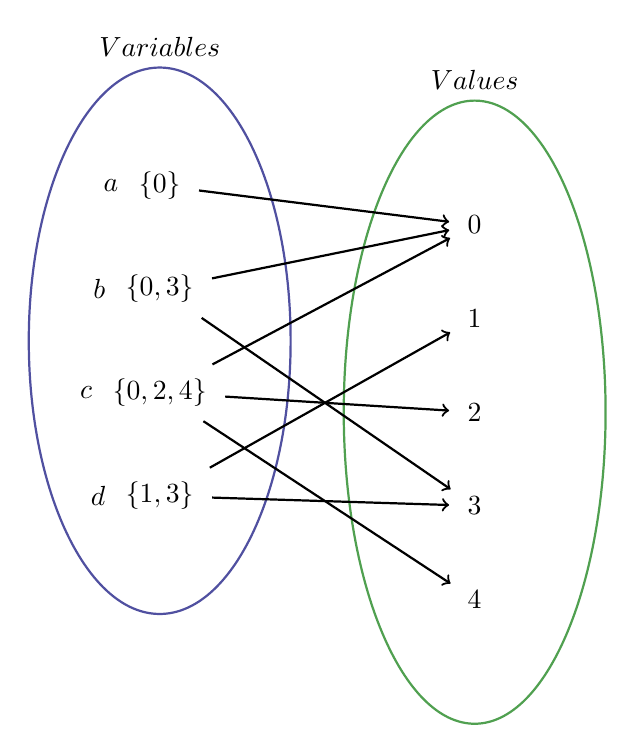
\begin{tikzpicture}[thick,
  fsnode/.style={},
  ssnode/.style={},
  every fit/.style={ellipse,draw,inner sep=5pt,text width=2cm},
  ->,shorten >= 3pt,shorten <= 3pt
]
% the vertices of U
\begin{scope}[start chain=going below,node distance=7mm]
  \node[fsnode,on chain,label=left:$a$] (a) {$\{0\}$};
  \node[fsnode,on chain,label=left:$b$] (b) {$\{0,3\}$};
  \node[fsnode,on chain,label=left:$c$] (c) {$\{0,2,4\}$};
  \node[fsnode,on chain,label=left:$d$] (d) {$\{1,3\}$};
\end{scope}

% the vertices of V
\begin{scope}[xshift=4cm,yshift=-0.5cm,start chain=going below,node distance=7mm]
  \node[ssnode,on chain] (v0) {$0$};
  \node[ssnode,on chain] (v1) {$1$};
  \node[ssnode,on chain] (v2) {$2$};
  \node[ssnode,on chain] (v3) {$3$};
  \node[ssnode,on chain] (v4) {$4$};
\end{scope}

% the set U
\node [myblue,fit=(a) (d),label=above:$Variables$] {};
% the set V
\node [mygreen,fit=(v0) (v4),label=above:$Values$] {};

% the edges
\draw (a) -- (v0);
\draw (b) -- (v0);
\draw (b) -- (v3);
\draw (c) -- (v0);
\draw (c) -- (v2);
\draw (c) -- (v4);
\draw (d) -- (v1);
\draw (d) -- (v3);

%%\draw (f1) [red]-- (s6);
\end{tikzpicture}
\end{figure}
\textbf{Find an initial matching:}
\begin{figure}[H]
\centering
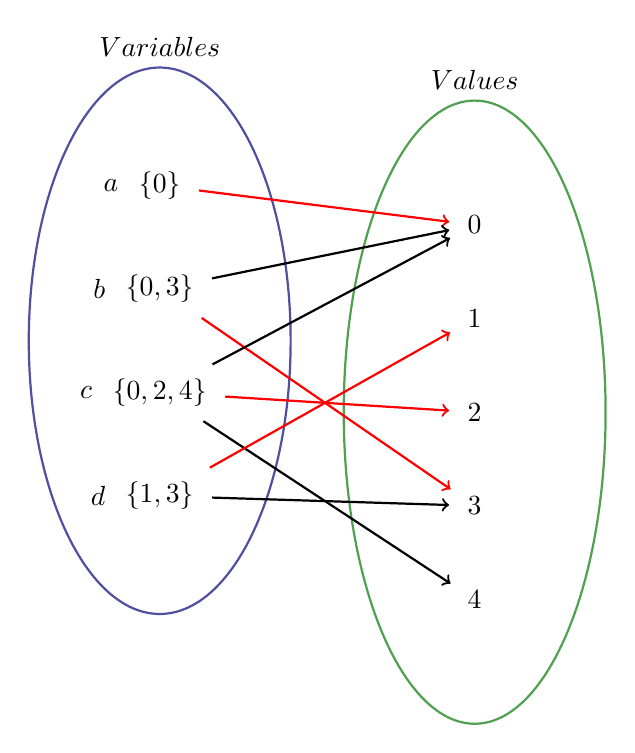
\begin{tikzpicture}[thick,
  fsnode/.style={},
  ssnode/.style={},
  every fit/.style={ellipse,draw,inner sep=5pt,text width=2cm},
  ->,shorten >= 3pt,shorten <= 3pt
]
% the vertices of U
\begin{scope}[start chain=going below,node distance=7mm]
  \node[fsnode,on chain,label=left:$a$] (a) {$\{0\}$};
  \node[fsnode,on chain,label=left:$b$] (b) {$\{0,3\}$};
  \node[fsnode,on chain,label=left:$c$] (c) {$\{0,2,4\}$};
  \node[fsnode,on chain,label=left:$d$] (d) {$\{1,3\}$};
\end{scope}

% the vertices of V
\begin{scope}[xshift=4cm,yshift=-0.5cm,start chain=going below,node distance=7mm]
  \node[ssnode,on chain] (v0) {$0$};
  \node[ssnode,on chain] (v1) {$1$};
  \node[ssnode,on chain] (v2) {$2$};
  \node[ssnode,on chain] (v3) {$3$};
  \node[ssnode,on chain] (v4) {$4$};
\end{scope}

% the set U
\node [myblue,fit=(a) (d),label=above:$Variables$] {};
% the set V
\node [mygreen,fit=(v0) (v4),label=above:$Values$] {};

% the edges
\draw (a) [red]-- (v0);
\draw (b) -- (v0);
\draw (b) [red]-- (v3);
\draw (c) -- (v0);
\draw (c) [red]-- (v2);
\draw (c) -- (v4);
\draw (d) [red]-- (v1);
\draw (d) -- (v3);

%%\draw (f1) [red]-- (s6);
\end{tikzpicture}
\end{figure}

\textbf{Orient edges for simplicity:}
\begin{figure}[H]
\centering
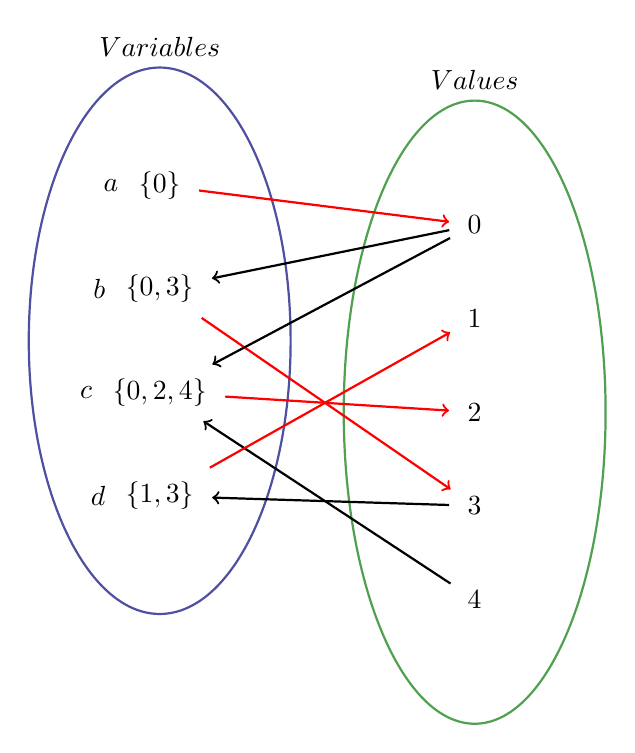
\begin{tikzpicture}[thick,
  fsnode/.style={},
  ssnode/.style={},
  every fit/.style={ellipse,draw,inner sep=5pt,text width=2cm},
  ->,shorten >= 3pt,shorten <= 3pt
]
% the vertices of U
\begin{scope}[start chain=going below,node distance=7mm]
  \node[fsnode,on chain,label=left:$a$] (a) {$\{0\}$};
  \node[fsnode,on chain,label=left:$b$] (b) {$\{0,3\}$};
  \node[fsnode,on chain,label=left:$c$] (c) {$\{0,2,4\}$};
  \node[fsnode,on chain,label=left:$d$] (d) {$\{1,3\}$};
\end{scope}

% the vertices of V
\begin{scope}[xshift=4cm,yshift=-0.5cm,start chain=going below,node distance=7mm]
  \node[ssnode,on chain] (v0) {$0$};
  \node[ssnode,on chain] (v1) {$1$};
  \node[ssnode,on chain] (v2) {$2$};
  \node[ssnode,on chain] (v3) {$3$};
  \node[ssnode,on chain] (v4) {$4$};
\end{scope}

% the set U
\node [myblue,fit=(a) (d),label=above:$Variables$] {};
% the set V
\node [mygreen,fit=(v0) (v4),label=above:$Values$] {};

% the edges
\draw (a) [red]-- (v0);
\draw (v0) -- (b);
\draw (b) [red]-- (v3);
\draw (v0) -- (c);
\draw (c) [red]-- (v2);
\draw (v4) -- (c);
\draw (d) [red]-- (v1);
\draw (v3) -- (d);

%%\draw (f1) [red]-- (s6);
\end{tikzpicture}
\end{figure}

\textbf{Find alternating paths and mark edges traversed through the path}

Start from free node and visit one node at a time on the path and we find the following alternating even paths starting at free node:

Free nodes are: $\{4\}$

Even alternating path starting at $4$ of length $2$:

$4 \rightarrow c \rightarrow 2$

Mark edge $(4, c)$ (edge $(c,2)$ already part of matching):

\begin{figure}[H]
\centering
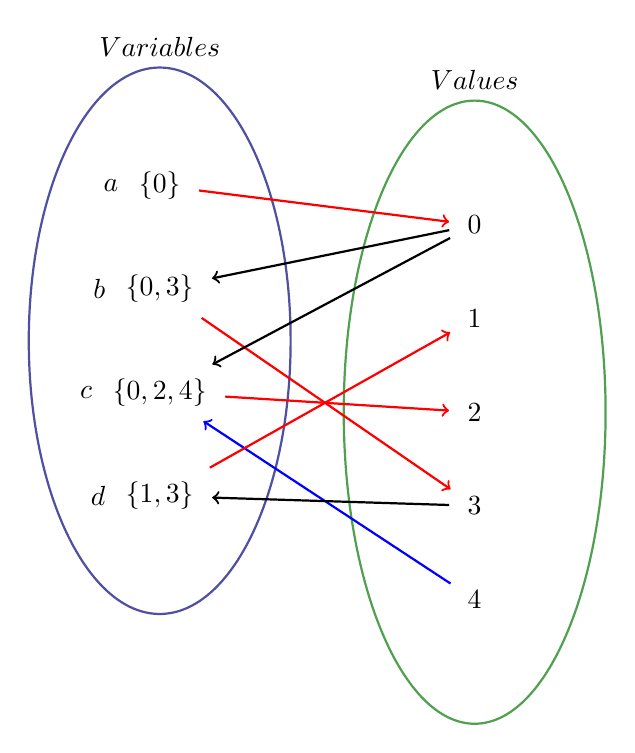
\begin{tikzpicture}[thick,
  fsnode/.style={},
  ssnode/.style={},
  every fit/.style={ellipse,draw,inner sep=5pt,text width=2cm},
  ->,shorten >= 3pt,shorten <= 3pt
]
% the vertices of U
\begin{scope}[start chain=going below,node distance=7mm]
  \node[fsnode,on chain,label=left:$a$] (a) {$\{0\}$};
  \node[fsnode,on chain,label=left:$b$] (b) {$\{0,3\}$};
  \node[fsnode,on chain,label=left:$c$] (c) {$\{0,2,4\}$};
  \node[fsnode,on chain,label=left:$d$] (d) {$\{1,3\}$};
\end{scope}

% the vertices of V
\begin{scope}[xshift=4cm,yshift=-0.5cm,start chain=going below,node distance=7mm]
  \node[ssnode,on chain] (v0) {$0$};
  \node[ssnode,on chain] (v1) {$1$};
  \node[ssnode,on chain] (v2) {$2$};
  \node[ssnode,on chain] (v3) {$3$};
  \node[ssnode,on chain] (v4) {$4$};
\end{scope}

% the set U
\node [myblue,fit=(a) (d),label=above:$Variables$] {};
% the set V
\node [mygreen,fit=(v0) (v4),label=above:$Values$] {};

% the edges
\draw (a) [red]-- (v0);
\draw (v0) -- (b);
\draw (b) [red]-- (v3);
\draw (v0) -- (c);
\draw (c) [red]-- (v2);
\draw (v4) [blue]-- (c);
\draw (d) [red]-- (v1);
\draw (v3) -- (d);

%%\draw (f1) [red]-- (s6);
\end{tikzpicture}
\end{figure}

\textbf{Find even alternating cycles and mark edges through the path}

There are no such cycles in this graph.

The cycles can be computed by first finding strongly connected components in the graph (strongly connected component is a component where there are pairwise paths from every node in the component). Mark the edges connecting the component. (Notice that there is no restriction of cycles starting at free nodes so that's why this technique will mark all edges in all even alternating cycles).

\textbf{Remove all unmarked edges from the graph}:

\begin{figure}[H]
\centering
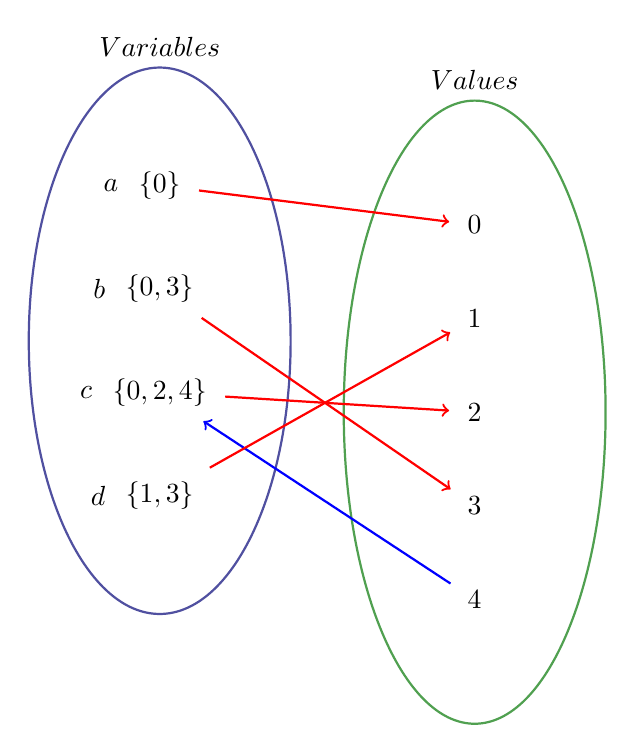
\begin{tikzpicture}[thick,
  fsnode/.style={},
  ssnode/.style={},
  every fit/.style={ellipse,draw,inner sep=5pt,text width=2cm},
  ->,shorten >= 3pt,shorten <= 3pt
]
% the vertices of U
\begin{scope}[start chain=going below,node distance=7mm]
  \node[fsnode,on chain,label=left:$a$] (a) {$\{0\}$};
  \node[fsnode,on chain,label=left:$b$] (b) {$\{0,3\}$};
  \node[fsnode,on chain,label=left:$c$] (c) {$\{0,2,4\}$};
  \node[fsnode,on chain,label=left:$d$] (d) {$\{1,3\}$};
\end{scope}

% the vertices of V
\begin{scope}[xshift=4cm,yshift=-0.5cm,start chain=going below,node distance=7mm]
  \node[ssnode,on chain] (v0) {$0$};
  \node[ssnode,on chain] (v1) {$1$};
  \node[ssnode,on chain] (v2) {$2$};
  \node[ssnode,on chain] (v3) {$3$};
  \node[ssnode,on chain] (v4) {$4$};
\end{scope}

% the set U
\node [myblue,fit=(a) (d),label=above:$Variables$] {};
% the set V
\node [mygreen,fit=(v0) (v4),label=above:$Values$] {};

% the edges
\draw (a) [red]-- (v0);
\draw (b) [red]-- (v3);
\draw (c) [red]-- (v2);
\draw (v4) [blue]-- (c);
\draw (d) [red]-- (v1);

%%\draw (f1) [red]-- (s6);
\end{tikzpicture}
\end{figure}

Now the algorithm is terminated and we have computed the store as result of propagation:

$p(s) = s' = \{a \mymapsto \{0\} b \mymapsto \{3\} c \mymapsto \{2, 4\} d \mymapsto \{1\}\}$
\bibliography{references}{}
\bibliographystyle{plain}
\end{document}